\documentclass[a4paper,french]{paper}
\usepackage{../../_latex_assets/villemejane_iogs_ceti}

%Informations about this document 
%------------------------------------------
\def\module{Conception Electronique pour le Traitement de l'Information}
\def\moduleAbrege{5N-027-SCI / CéTI}
\def\annee{}

\def\titre{Bloc 1 / Capteurs et mise en forme}
\author{Julien VILLEMEJANE}

\subtitle{Bloc 1}
\institution{LEnsE / Institut d'Optique Graduate School}

\title{\titre}
\begin{document} 
%Beginning First Page. 
%------------------------------------------
\enteteThematiqueObligatoire{}

%Beginning Content. 
%------------------------------------------

%%%%%%%%%%%%%%%%%%%
\encadreTDExo{1.1 - Abaisser une tension}{
Proposer un circuit permettant d'abaisser une tension d'un facteur $k$.

$0 < k < 1$ 
}

%%%%%%%%%%%%%%%%%%%
\encadreTDExo{1.2 - Élever une tension}{
Proposer un circuit permettant d'élever une tension d'un facteur $k$.

$k > 1$
}

%%%%%%%%%%%%%%%%%%%
\encadreTDExo{1.3 - Limiter une tension}{
Rappeler le fonctionnement d'une diode.

Décrire le fonctionnement du montage suivant :

\begin{center}
\begin{circuitikz}
	\draw (0,0) to[battery2, invert] (0,5) to[short, -] (6,5)
		to[full diode=$D_1$, invert, i<_=$i_1$	] (6,2.5) to[full diode=$D_2$, invert, i<_=$i_2$, *-] (6,0)
		to[short, -*] (3,0) node[ground](GND){} to[short, -] (0,0);
	\draw (3,0) to[sV] (3,2.5) to[R=$R_p$, i=$i_R$] (6,2.5);
	\draw (6,2.5) to[short, -o] (8,2.5);
	\draw (8, 0) to[short, -o] ++(0,0) node[ground](GND){};
	\draw (8,0.3) edge[->,color={red}] (8, 2.2);
	\node[text={red}] (Vs) at (8.5,1.3){$V_S$}; 
	\draw (7,0.3) edge[<-,color={blue}] (7, 2.2);
	\node[text={blue}] (Vd2) at (7.5,1.3){$V_{D2}$}; 
	\draw (7,4.7) edge[->,color={blue}] (7, 2.8);
	\node[text={blue}] (Vd1) at (7.5,3.7){$V_{D1}$}; 
	\draw (2.5,0.3) edge[->,color={green!40!black}] (2.5, 2.2);
	\node[text={green!40!black}] (Ve) at (2,1.3){$V_e$}; 
	\draw (0.7,0.3) edge[->,color={black}] (0.7, 4.7);
	\node[text={black}] (Vcc) at (1.3, 2.5){$V_{CC}$}; 
\end{circuitikz}
\end{center}

}

%%%%%%%%%%%%%%%%%%%
\encadreTDExo{1.4 - Amplifier un signal}{
Proposer un circuit permettant d'amplifier un signal de $27dB$, tout en garantissant une bande-passante de $400 kHz$.

On utilisera des amplificateurs linéaires intégrés de type TL071 (documentation partielle donnée en annexe).
}


%%%%%%%%%%%%%%%%%%%
\encadreTDExo{1.5 - Additionner des signaux}{
On se propose d'étudier le circuit suivant :
\begin{center}
	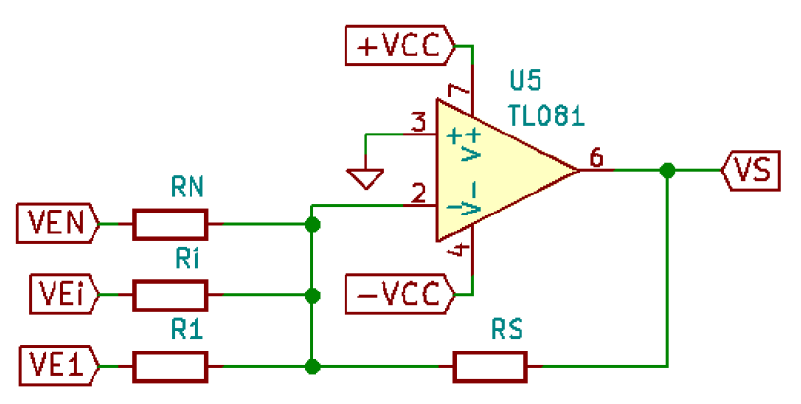
\includegraphics[width=10cm]{images/ali_ampli_somme.png}
\end{center}
}


%%%%%%%%%%%%%%%%%%%
\encadreTDExo{1.6 - Mettre en forme un capteur de température}{
On se propose d'étudier le circuit suivant :

\begin{center}
	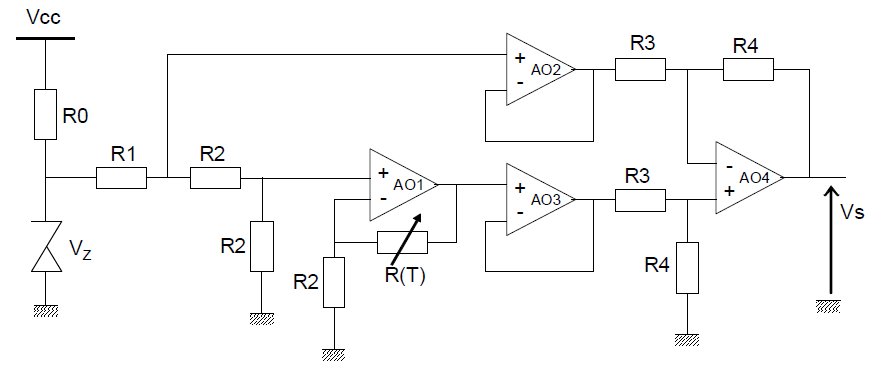
\includegraphics[width=16cm]{images/capteur_conditionnement.png}
\end{center}

La thermistance utilisée est de type PT100. La relation entre sa résistance (en Ohms) et la température (en \degre{}C) est la suivante :
$$R(T) = 100~(1 + 3.908×10^{-3} T - 5.802×10^{-7} T^2)$$

Une partie de la documentation de diodes Zener est fournie en annexe.
}

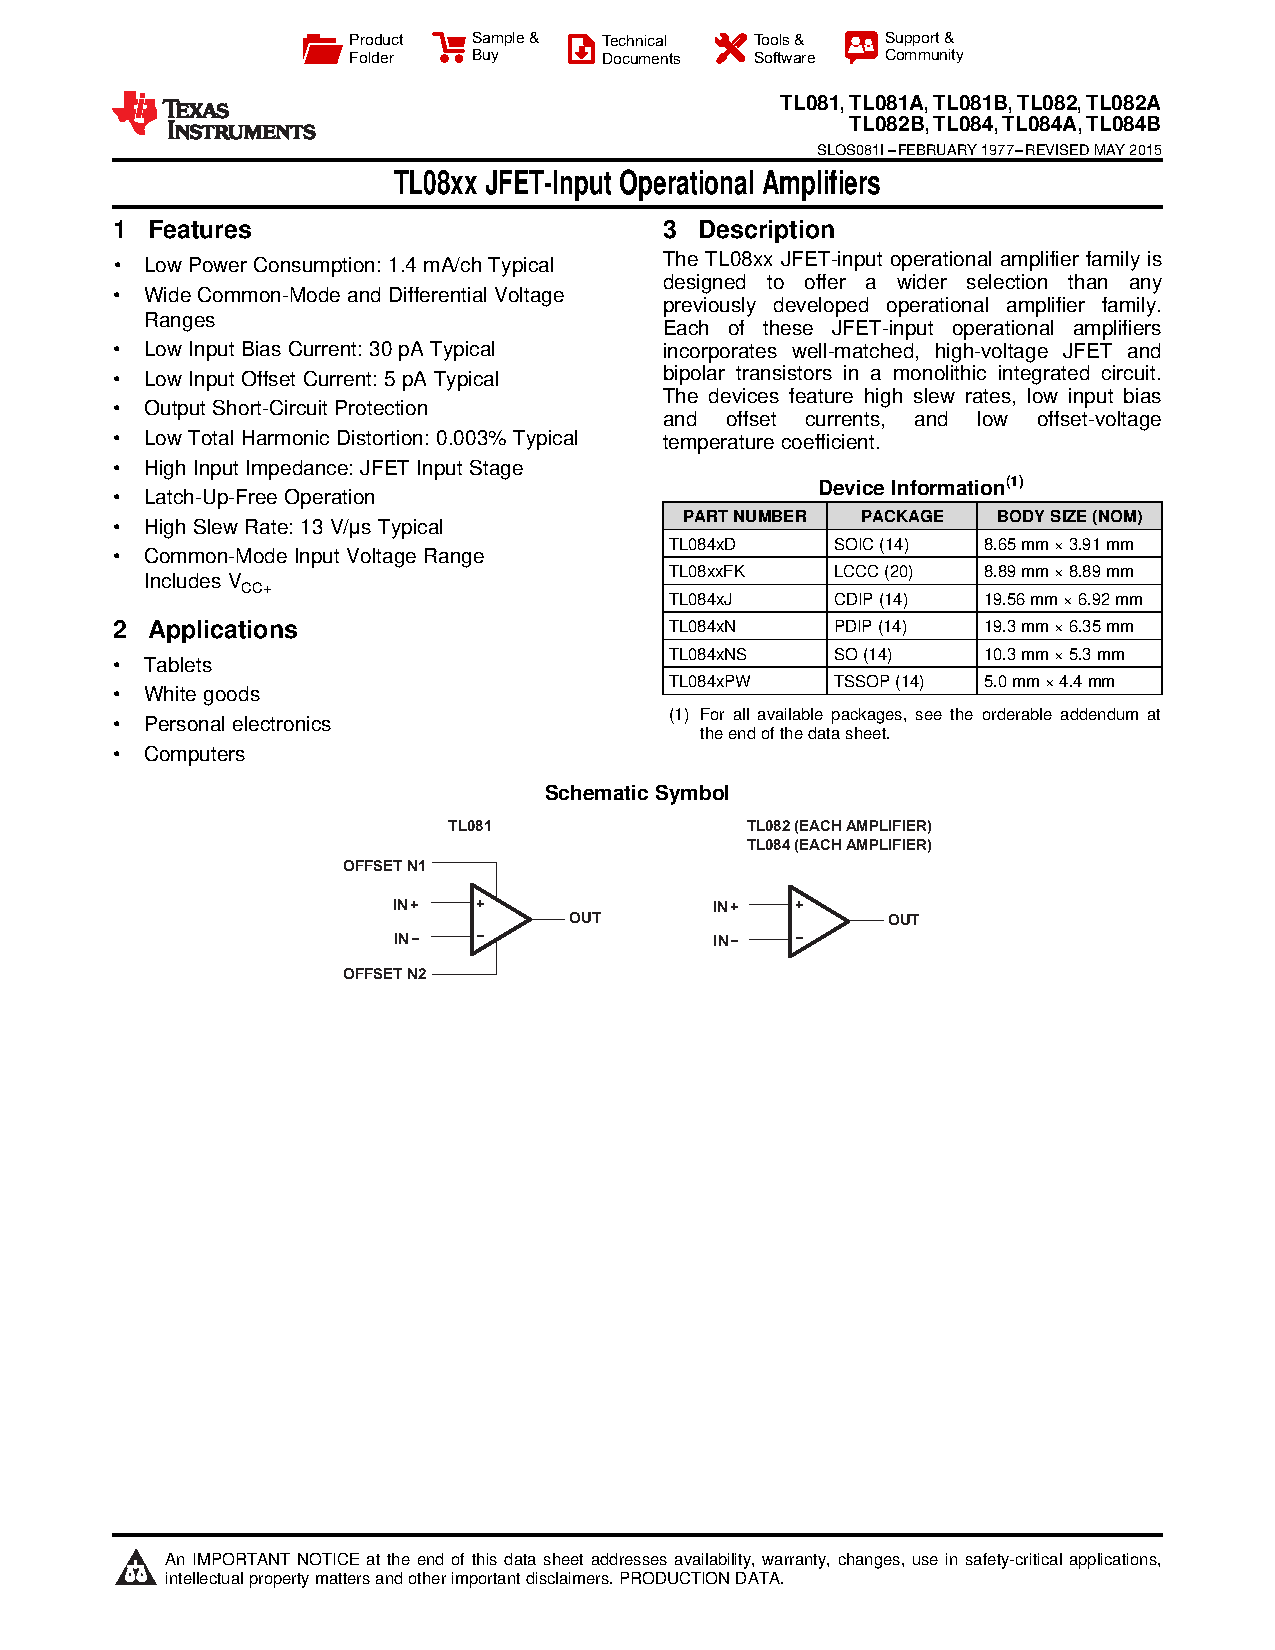
\includepdf[pages=-]{doc/doc_TL071_1p.pdf}
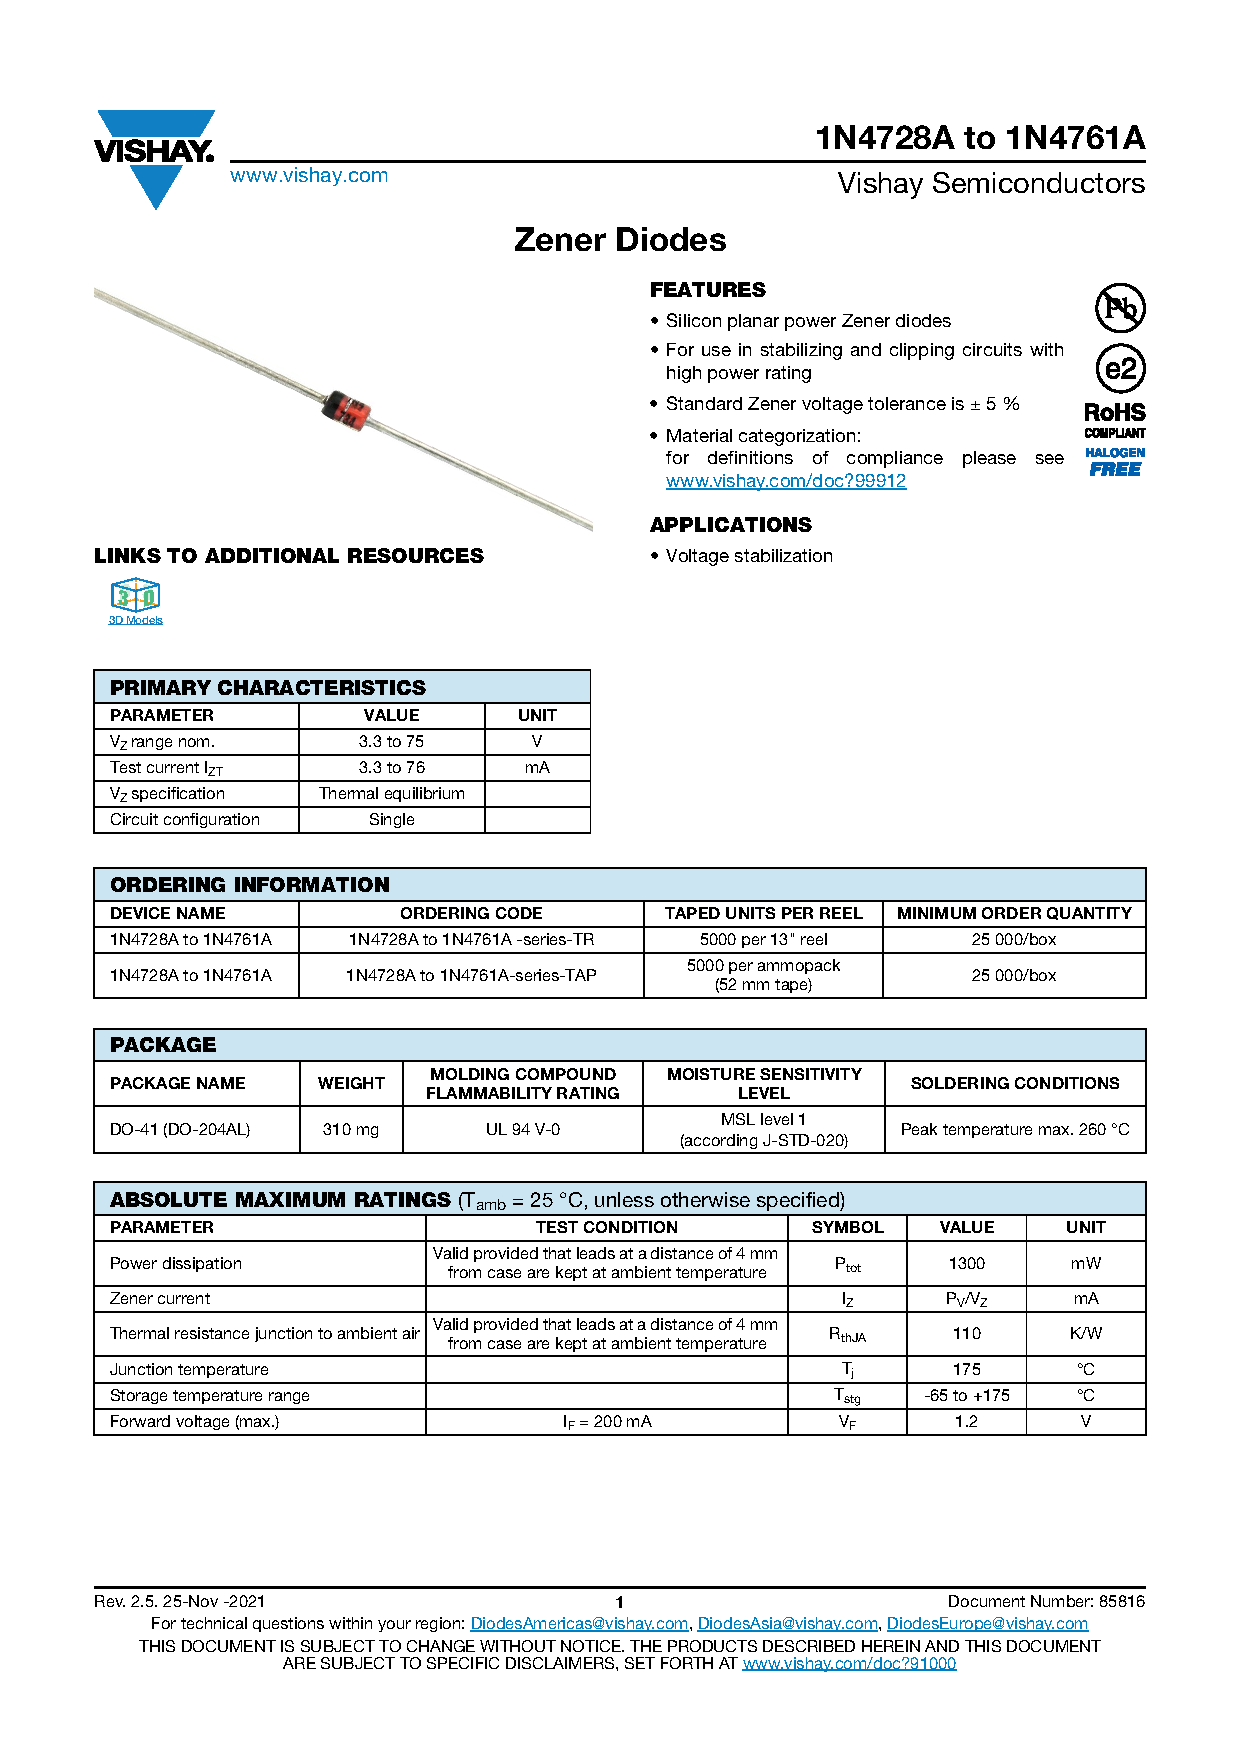
\includepdf[pages=1-2]{doc/1n4728a.pdf}

\end {document}